\documentclass[11pt,a4paper]{article}
\usepackage[utf8]{inputenc}
\usepackage[T1]{fontenc}
\IfFileExists{lmodern.sty}{\usepackage{lmodern}}{}
\usepackage[margin=2.3cm]{geometry}
\usepackage{amsmath,amssymb,bm,mathtools}
\usepackage{graphicx}
\usepackage{booktabs}
\usepackage{multirow}
\usepackage{xcolor}
\usepackage{tikz}
\usetikzlibrary{positioning,arrows.meta}
\usepackage{caption}
\usepackage{enumitem}
\usepackage[hidelinks]{hyperref}
\usepackage{xurl}
\usepackage{float}

\graphicspath{{figures/}}
\newcommand{\todo}[1]{\textcolor{red}{[#1]}}
\newcommand{\vect}[1]{\bm{#1}}
\setlist{itemsep=2pt,topsep=4pt}

\title{\textbf{Gaussian Splatting for Physical Inverse Problems}\\[4pt]
\large MS Thesis I --- Progress Report}
\author{Muhammad Hussain Qureshi \quad \todo{Roll no.}\\
Advisor: \todo{Advisor name}\\
Faculty of Sciences, Information Technology University, Lahore}
\date{November 8, 2026}

\begin{document}
\maketitle

\begin{abstract}
\noindent We use Gaussian Splatting as a representation for physical fields that are observed only through a known
forward model, using datasets and operators from InverseBench. 3D Gaussians reconstruct cells from scattered
electromagnetic fields (inverse scattering), and 4D Gaussians with an MLP or Mamba deformation network reconstruct
2D Navier--Stokes flow over time from sparse observations. All three planned experiments run end to end, the code is
in a structured GitHub repository, and the thesis document is drafted. This report summarises the method, the
results (including negative ones), the new true 3D scattering model, sharper kernels and a ten-cell evaluation, and
questions for the next meeting.
\end{abstract}

\section{Status at a glance}
\begin{table}[H]
\centering
\begin{tabular}{p{6.3cm}p{2.3cm}p{6.3cm}}
\toprule
Item & Status & Note \\
\midrule
3D Gaussians on inverse scattering (2D and 3D) & done & 2D cells, synthetic and real (BBBC024) 3D nuclei \\
4D Gaussians on Navier--Stokes & done & held-out frames, 100\% and 10\% observations \\
Mamba as the motion model & done & MLP vs.\ Mamba vs.\ bidirectional Mamba \\
True 3D scattering model & done & sensors on a sphere; grid wins (Section~\ref{sec:running}) \\
Sharper (generalised) Gaussian kernels & done & did not help under the physics loss \\
More samples with spread (10 cells) & done & paired comparison, mean $\pm$ std \\
GitHub repository (standard structure) & done & to be transferred to the thesis account \\
Thesis document (LaTeX, 40 pages) & draft & all required chapters \\
Slides and Open House poster (A0) & draft & updated with all results \\
\bottomrule
\end{tabular}
\end{table}

\section{Method}
\paragraph{Representation.} A field $f$ on a grid is a sum of anisotropic Gaussians,
\begin{equation}
f_\Theta(\vect{x}) = \sum_{i=1}^{N} a_i \exp\!\Big(-\tfrac12\big[(\vect{x}-\vect{\mu}_i)^\top \Sigma_i^{-1}(\vect{x}-\vect{\mu}_i)\big]^{\beta}\Big),
\qquad \Sigma_i = R_i S_i^2 R_i^\top ,
\end{equation}
with position $\vect{\mu}_i$, scales $S_i$, rotation $R_i$ (angle in 2D, quaternion in 3D) and amplitude $a_i\ge0$
(signed for vorticity). $\beta=1$ is the usual Gaussian; $\beta>1$ gives flatter tops and sharper edges. Each
Gaussian is evaluated only in a local window around its centre, as in 3DGS.

\paragraph{Physics instead of a camera.} The camera rasteriser of 3DGS is replaced by the forward operator
$\mathcal{A}$ of the problem (Figure~\ref{fig:pipeline}). Parameters are fitted with Adam to
\begin{equation}
\min_\Theta\ \frac{\lVert \mathcal{A} f_\Theta - \vect{y}\rVert_2^2}{\lVert \vect{y}\rVert_2^2} + \lambda\,\overline{f_\Theta},
\end{equation}
where the second term is a sparsity penalty on the mean intensity. New Gaussians are added where the back-projected
residual $\operatorname{Re}\mathcal{A}^{H}(\vect{y}-\mathcal{A}f_\Theta)$ is largest; Gaussians with negligible
amplitude are pruned. The baseline optimises every pixel or voxel directly with the same loss.

\paragraph{Inverse scattering.} The linear (Born) model of InverseBench:
$y_{t,r} = \Delta x\,\Delta y \sum_p f_p\, \overline{u^{\mathrm{inc}}_{p,t}}\, G_{p,r}$, with 20 transmitters and 360, 180
or 60 receivers on a circle (our implementation matches InverseBench to $3\times10^{-7}$). For 3D volumes the
operator was first applied slice by slice. The new \emph{true 3D} model (Section~\ref{sec:running}) uses 3D Green's
functions with sensors on a sphere.

\paragraph{4D Gaussians for flow.} Canonical Gaussians are moved over time by a deformation network
$\Delta\vect{\mu}_i(t), \Delta s_i(t), \Delta a_i(t) = D_\phi(\vect{\mu}_i, t)$: an MLP with Fourier features
(as in 4D Gaussian Splatting) or a Mamba selective state-space model that reads each Gaussian's trajectory over
all time steps as a sequence (causal or bidirectional). A temporal smoothness term
$\lambda_T \sum_t \lVert D_\phi(\cdot,t{+}1) - D_\phi(\cdot,t)\rVert^2$ links observed and unobserved times.

\begin{figure}[H]
\centering
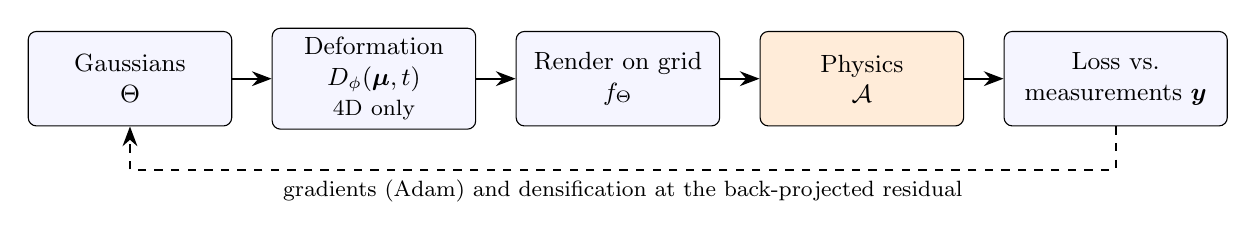
\begin{tikzpicture}[
  box/.style={draw, rounded corners=3pt, align=center, minimum height=1.2cm, text width=2.35cm, font=\small, fill=blue!4},
  dark/.style={box, fill=orange!15},
  arr/.style={-{Stealth[length=2.5mm]}, thick}, node distance=0.5cm]
  \node[box] (g) {Gaussians\\$\Theta$};
  \node[box, right=of g] (d) {Deformation\\$D_\phi(\vect\mu,t)$\\{\footnotesize 4D only}};
  \node[box, right=of d] (r) {Render on grid\\$f_\Theta$};
  \node[dark, right=of r] (a) {Physics\\$\mathcal{A}$};
  \node[box, right=of a, text width=2.6cm] (l) {Loss vs.\\measurements $\vect{y}$};
  \draw[arr] (g) -- (d); \draw[arr] (d) -- (r); \draw[arr] (r) -- (a); \draw[arr] (a) -- (l);
  \draw[arr, dashed] (l.south) -- ++(0,-0.55) -| node[pos=0.25, below, font=\footnotesize]{gradients (Adam) and densification at the back-projected residual} (g.south);
\end{tikzpicture}
\caption{Pipeline: the camera of Gaussian Splatting is replaced by the physics operator.}
\label{fig:pipeline}
\end{figure}

\section{Results so far}
All runs: NVIDIA T4, 3000 iterations, InverseBench noise level. PSNR in dB / SSIM, means over samples.

\subsection{2D inverse scattering (InverseBench cells)}
Without regularisation, adding Gaussians made results \emph{worse}: they grew ghost copies of the cell in regions the
receivers cannot see (the operator's null space, Figure~\ref{fig:ghost}). A sparsity term removes the ghosts. With
it, Gaussians beat the plain pixel grid in SSIM at 60 receivers, but a pixel grid given the same sparsity term
matches or beats the Gaussians (Table~\ref{tab:s2d}): the gain comes from the prior, not from the representation.

\begin{table}[H]
\centering
\caption{2D inverse scattering, 5 cells (PSNR / SSIM).}
\label{tab:s2d}
\begin{tabular}{lccc}
\toprule
Method & 360 receivers & 180 receivers & 60 receivers \\
\midrule
Gaussians, no sparsity (3 cells) & 30.7 / 0.959 & 30.4 / 0.957 & 26.5 / 0.814 \\
Gaussians + sparsity ($\lambda=0.3$) & 30.8 / 0.980 & 30.6 / 0.979 & 27.1 / 0.924 \\
Pixel grid & \textbf{36.1} / 0.984 & \textbf{34.7} / 0.974 & \textbf{28.6} / 0.886 \\
Pixel grid + sparsity ($\lambda=0.3$) & 33.2 / \textbf{0.985} & 32.5 / \textbf{0.983} & 27.7 / \textbf{0.933} \\
\bottomrule
\end{tabular}
\end{table}

\begin{figure}[H]
\centering
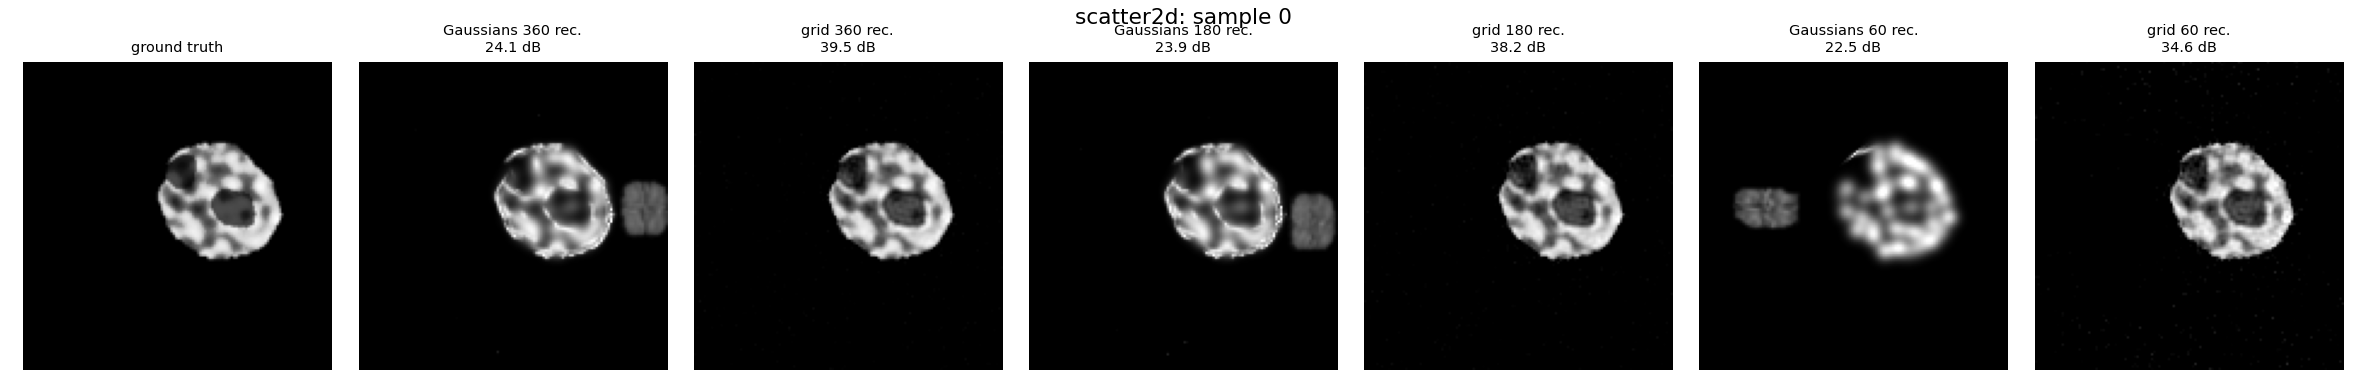
\includegraphics[width=\linewidth]{scatter2d_ghost.png}\\[2pt]
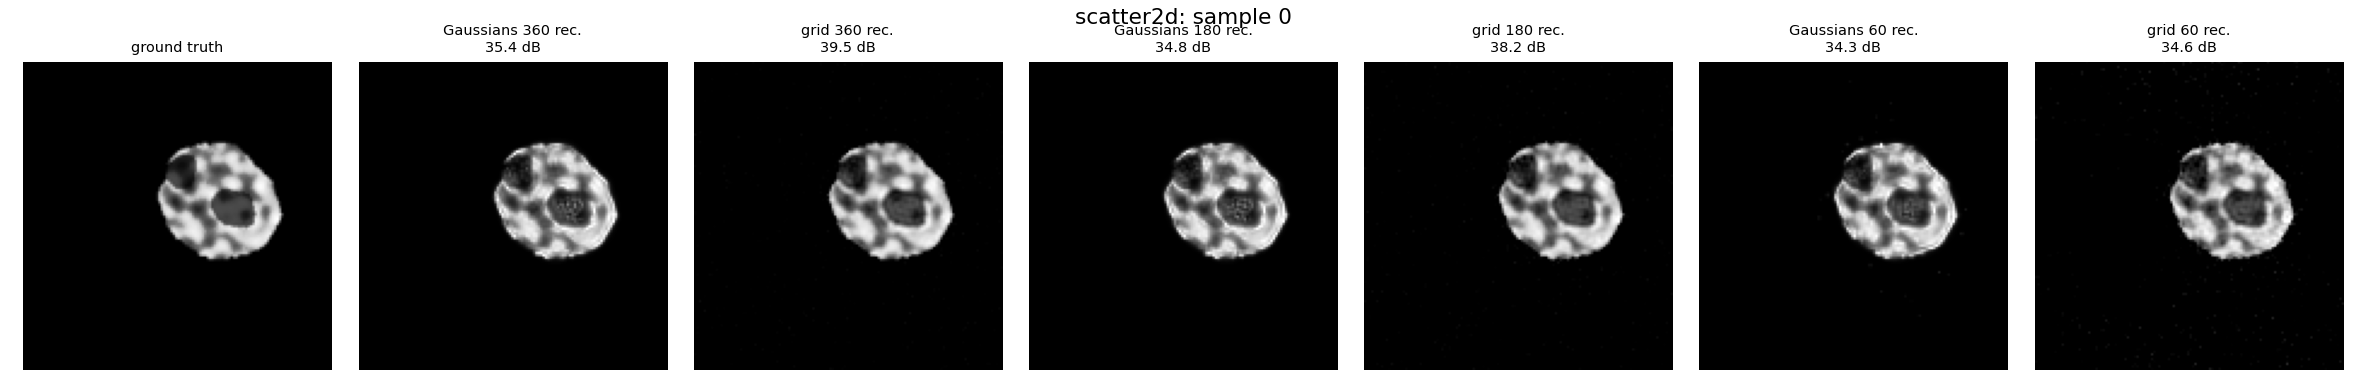
\includegraphics[width=\linewidth]{scatter2d_sparsity.png}
\caption{Cell 0. Top: aggressive densification, no sparsity: a ghost copy appears beside the cell. Bottom: with
sparsity the ghost is gone. Columns: truth, then Gaussians and pixel grid at 360, 180 and 60 receivers.}
\label{fig:ghost}
\end{figure}

\subsection{3D inverse scattering (slice-wise operator)}
On smooth synthetic nuclei, Gaussians barely change as receivers drop (40.8 $\to$ 40.9\,dB) while the voxel grid
falls to 37.3\,dB and becomes speckled. On real BBBC024 nuclei, which are binary masks with sharp boundaries,
Gaussians stay near 27--28\,dB while voxels reach 35--42\,dB: smooth kernels soften the edges
(Table~\ref{tab:s3d}, Figure~\ref{fig:s3d}).

\begin{table}[H]
\centering
\caption{3D inverse scattering, $32\times128\times128$ volumes, 3 volumes (PSNR / SSIM).}
\label{tab:s3d}
\begin{tabular}{llccc}
\toprule
Volumes & Method & 360 receivers & 180 receivers & 60 receivers \\
\midrule
\multirow{2}{*}{Synthetic} & Gaussians & 40.8 / \textbf{0.994} & 40.6 / \textbf{0.994} & \textbf{40.9 / 0.988} \\
 & Voxel grid & \textbf{44.1} / 0.987 & \textbf{41.5} / 0.977 & 37.3 / 0.932 \\
\midrule
\multirow{4}{*}{BBBC024} & Gaussians & 27.9 / 0.967 & 27.6 / 0.965 & 27.0 / 0.943 \\
 & Voxel grid & \textbf{41.8} / 0.989 & \textbf{40.3} / 0.980 & \textbf{35.3} / 0.936 \\
 & Gaussians + sparsity & 28.4 / 0.974 & 28.4 / 0.974 & 27.4 / 0.955 \\
 & Voxel grid + sparsity & 38.5 / \textbf{0.996} & 38.0 / \textbf{0.995} & 34.4 / \textbf{0.971} \\
\bottomrule
\end{tabular}
\end{table}

\begin{figure}[H]
\centering
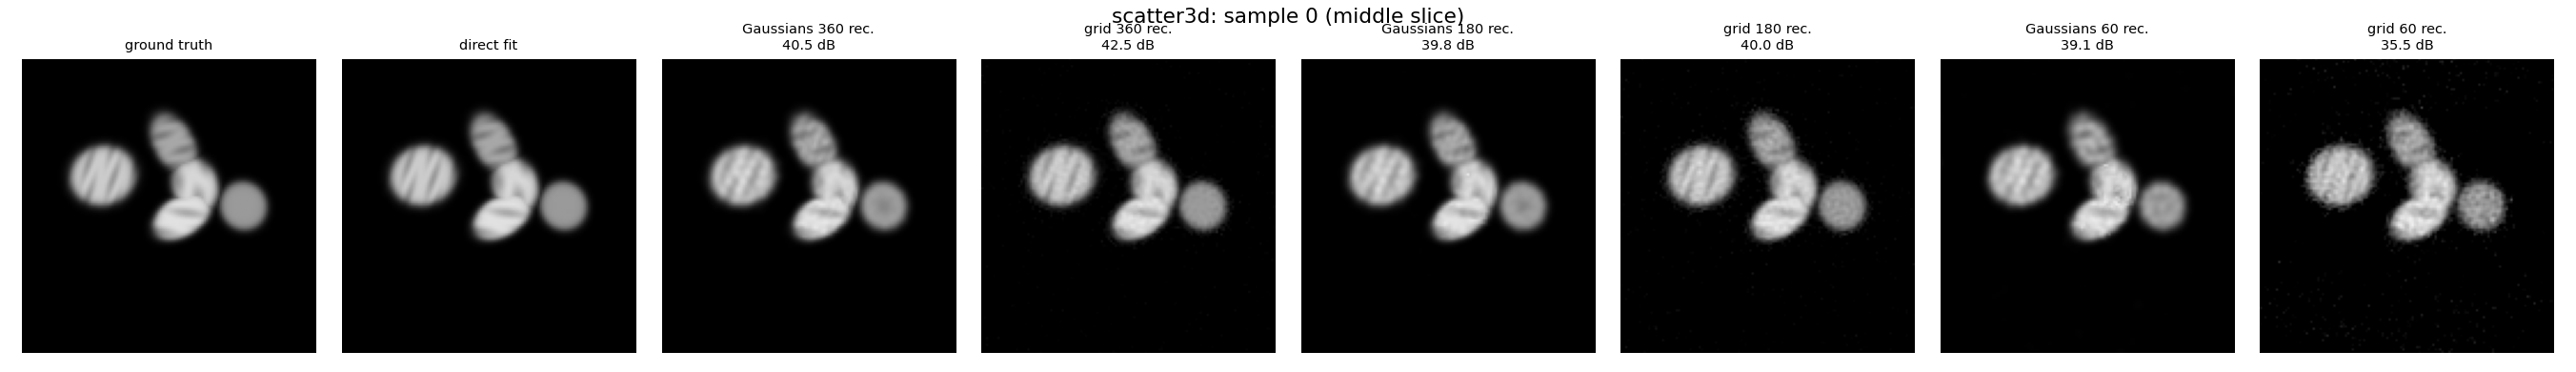
\includegraphics[width=\linewidth]{scatter3d_first.png}\\[2pt]
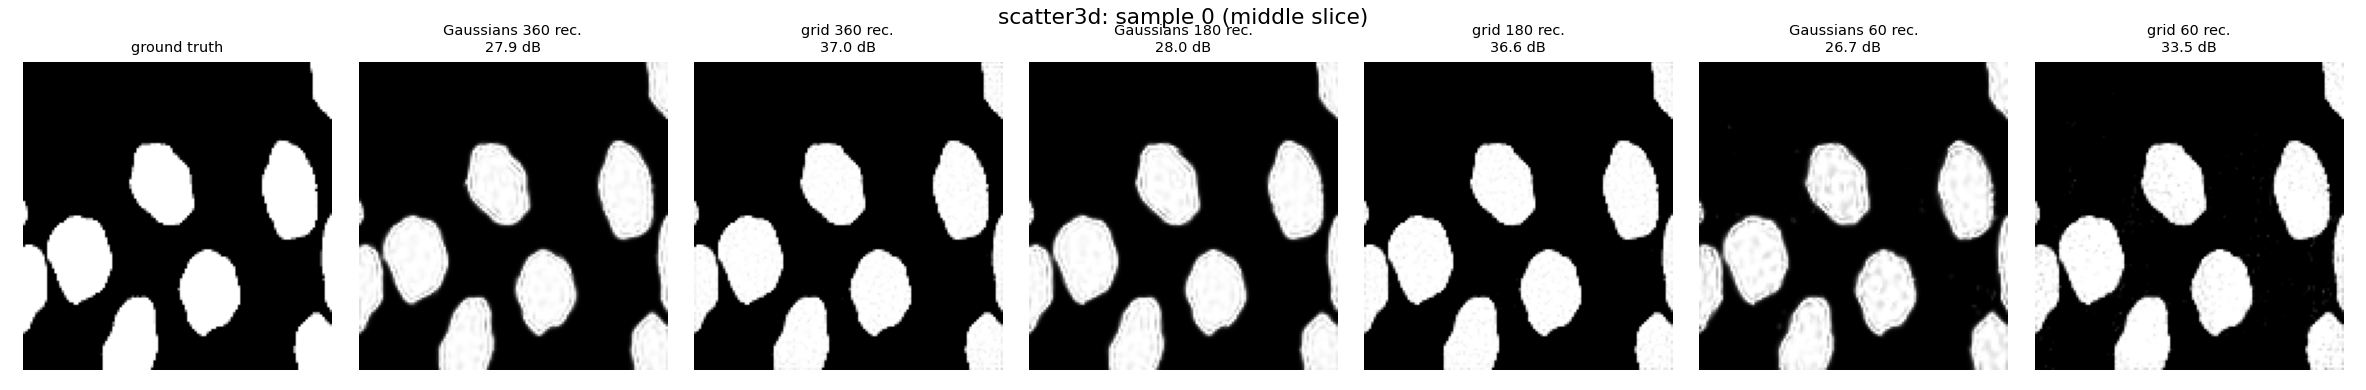
\includegraphics[width=\linewidth]{scatter3d_bbbc024.png}
\caption{Middle slices. Top: synthetic volume (truth, direct fit, then Gaussians and voxels at 360/180/60
receivers); voxels become speckled at 60 receivers. Bottom: BBBC024 volume; Gaussians soften the sharp boundaries.}
\label{fig:s3d}
\end{figure}

\subsection{4D Navier--Stokes}
Static Gaussians reach only 17\,dB; a deformation network adds about 10\,dB. Without regularisation, Mamba fits
observed frames much better than the MLP but does not generalise better to unseen times. With temporal smoothness,
Mamba beats the MLP by 2.4\,dB on unseen frames when only 10\% of pixels are observed, on each of the three sequences
(Table~\ref{tab:ns}, Figure~\ref{fig:ns}). The bidirectional variant gives no further gain and is twice as slow.

\begin{table}[H]
\centering
\caption{4D Navier--Stokes, PSNR (dB) on held-out frames; observed-frame PSNR in brackets; 3 sequences.}
\label{tab:ns}
\begin{tabular}{lcccc}
\toprule
Observed pixels & Static & MLP & Mamba & Bidirectional Mamba \\
\midrule
100\% & 17.0 (16.8) & 27.6 (30.3) & \textbf{27.9} (36.1) & -- \\
100\% + smoothness & -- & 27.4 (30.6) & 27.2 (35.2) & 26.4 (36.5) \\
10\% & 16.0 (15.9) & 23.2 (24.0) & 23.1 (27.7) & -- \\
10\% + smoothness & -- & 23.0 (24.1) & \textbf{25.4} (28.9) & 25.1 (29.6) \\
\midrule
Time per sequence & 3 min & 3 min & 15--28 min & 52 min \\
\bottomrule
\end{tabular}
\end{table}

\begin{figure}[H]
\centering
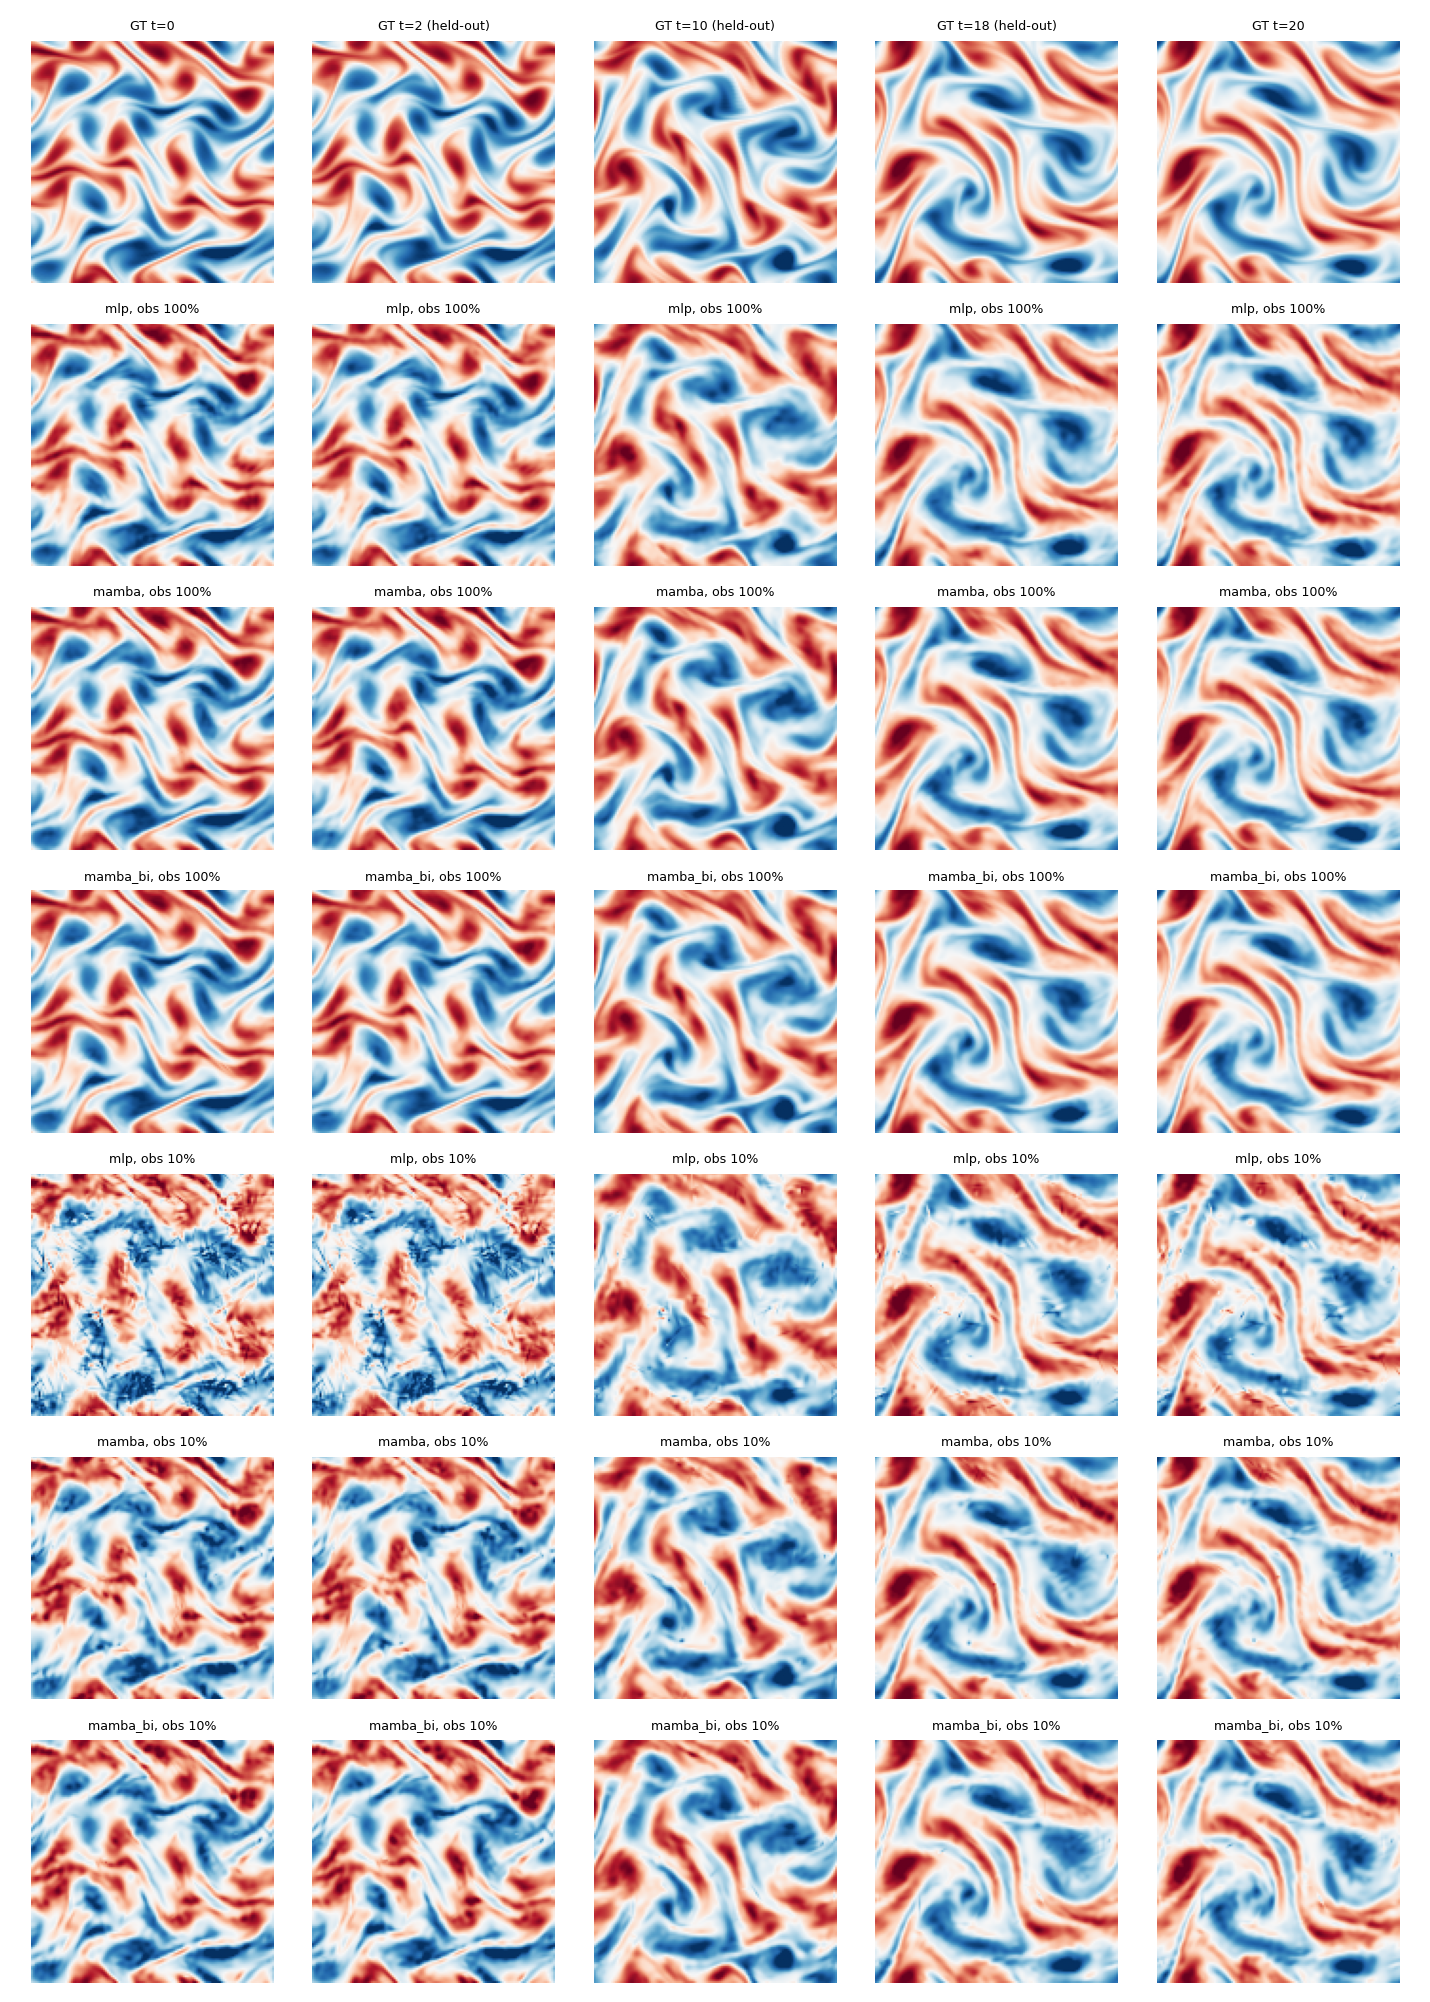
\includegraphics[width=0.72\linewidth]{ns4d_smooth.png}
\caption{Vorticity of sequence 0 at $t=0,2^*,10^*,18^*,20$ ($^*$ never observed). Rows: truth; MLP, Mamba and
bidirectional Mamba with 100\% and then 10\% of pixels observed. With 10\% the MLP shows streaks; Mamba stays coherent.}
\label{fig:ns}
\end{figure}

\section{New: true 3D model, sharper kernels, ten cells}
\label{sec:running}
\paragraph{True 3D scattering.} Following your request, the slice-wise operator is replaced by a first-order Born
model in 3D,
\begin{equation}
y_{t,r} = k^2\,\Delta V \sum_p f_p\, G(\lVert\vect{x}_t-\vect{x}_p\rVert)\, G(\lVert\vect{x}_r-\vect{x}_p\rVert),
\qquad G(d) = \frac{e^{\mathrm{i}kd}}{4\pi d},
\end{equation}
with the same voxel size, wavelength and sensor radius as InverseBench, 60 transmitters and 360/180/60 receivers
spread evenly over a sphere around the volume, and noise at the SNR of the 2D benchmark. The implementation matches
the analytic response of a point scatterer to $10^{-7}$ and passes an adjoint test. With about ten times fewer
measurements than the slice-wise model, the voxel grid is better than Gaussians in every setting
(Table~\ref{tab:born3d}). On BBBC024, Gaussians leave a bright rim at each boundary and under-fill the interior
(Figure~\ref{fig:born3d}); the voxel grid benefits from being clipped to $[0,1]$, a strong prior for binary objects
that Gaussians lack. Gaussians are, however, 11--12 times more compact.

\begin{table}[H]
\centering
\caption{True 3D scattering, $32\times128\times128$, sparsity 0.3 for both methods, 3 volumes (PSNR / SSIM).}
\label{tab:born3d}
\begin{tabular}{llcccc}
\toprule
Volumes & Method & Params & 360 rec. & 180 rec. & 60 rec. \\
\midrule
\multirow{2}{*}{Synthetic} & Gaussians & 42k & 37.6 / 0.977 & 36.6 / 0.955 & 32.1 / 0.852 \\
 & Voxel grid & 524k & \textbf{42.1 / 0.985} & \textbf{39.9 / 0.976} & \textbf{38.2 / 0.966} \\
\midrule
\multirow{3}{*}{BBBC024} & Gaussians & 47k & 25.6 / 0.960 & 24.9 / 0.940 & 20.9 / 0.772 \\
 & Gaussians, $\beta=4$ & 51k & 24.2 / 0.954 & 22.6 / 0.927 & 16.3 / 0.722 \\
 & Voxel grid & 524k & \textbf{32.5 / 0.983} & \textbf{30.5 / 0.956} & \textbf{25.6 / 0.875} \\
\bottomrule
\end{tabular}
\end{table}

\begin{figure}[H]
\centering
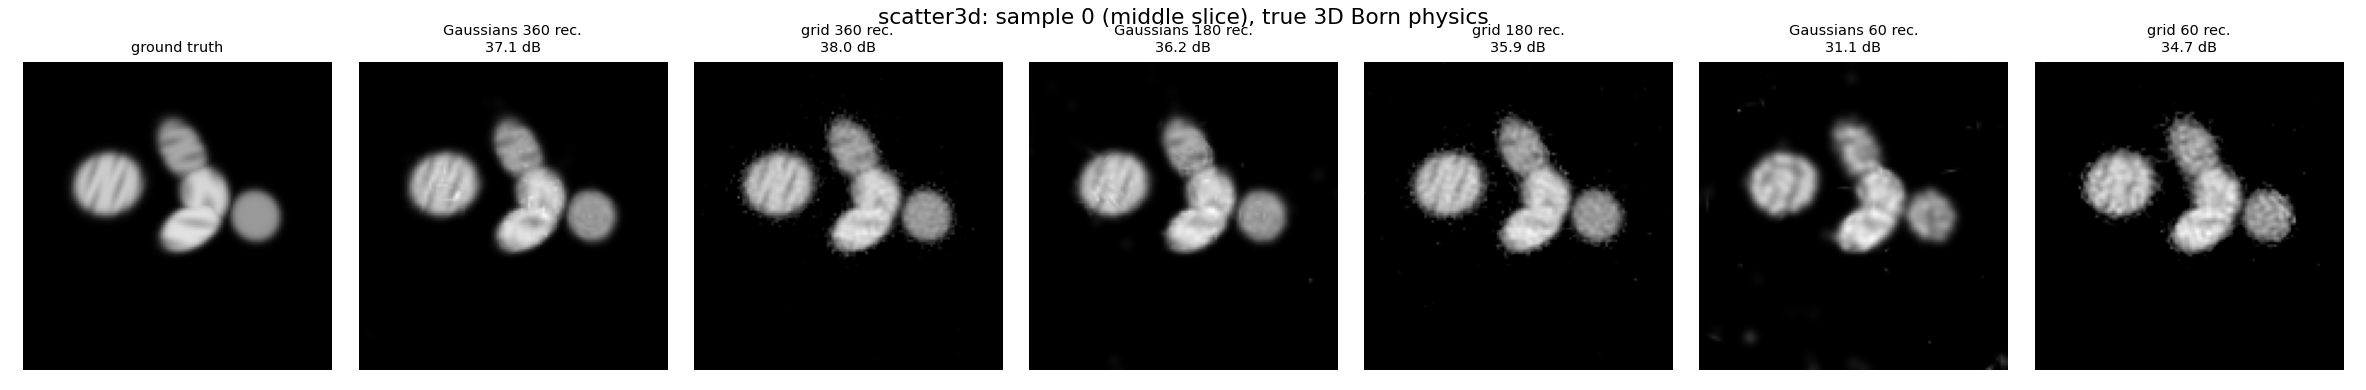
\includegraphics[width=\linewidth]{born3d_synthetic.png}\\[2pt]
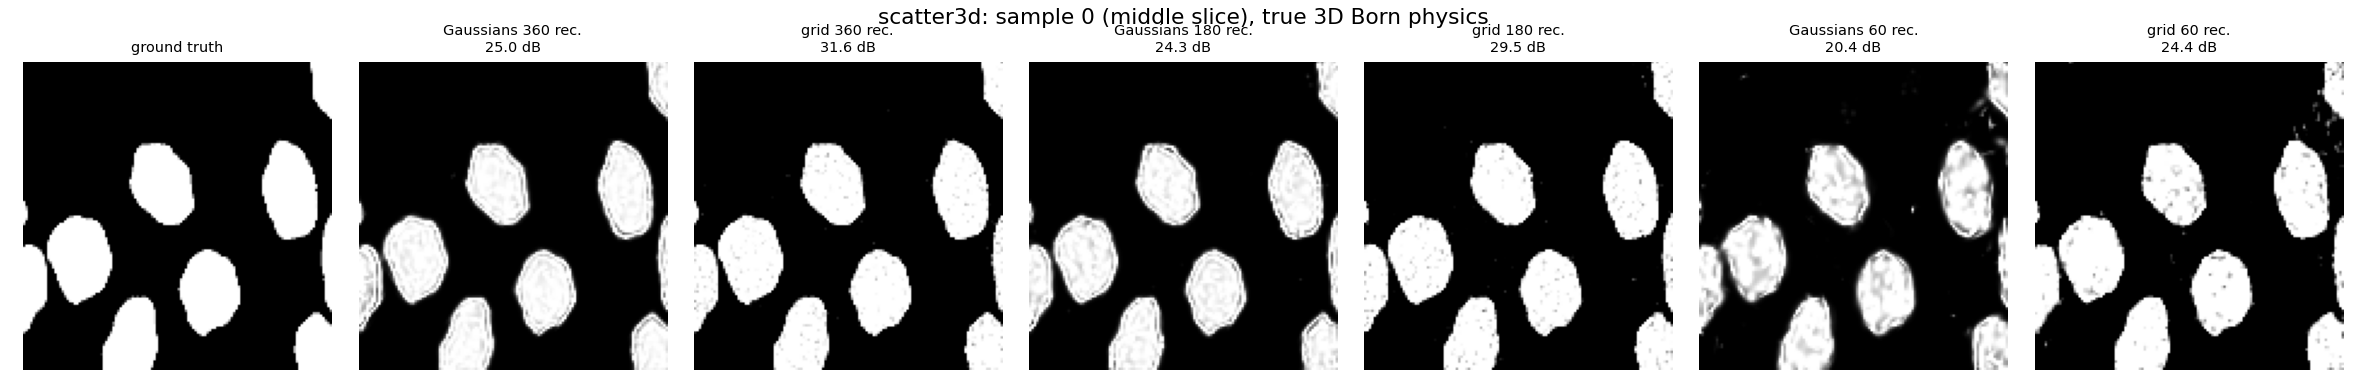
\includegraphics[width=\linewidth]{born3d_bbbc024.png}
\caption{True 3D model, middle slices. Top: synthetic nuclei. Bottom: BBBC024. Columns: truth, then Gaussians and
voxel grid at 360, 180 and 60 receivers.}
\label{fig:born3d}
\end{figure}

\paragraph{Sharper kernels.} Generalised Gaussians ($\beta=4$) fit binary masks about 3\,dB better when fitted
directly, but under the physics loss they are slightly worse (slice-wise BBBC024: 28.1 / 28.0 / 25.5\,dB vs.\
28.4 / 28.4 / 27.4\,dB).

\paragraph{Ten cells, paired.} In 2D, the pixel grid with the same sparsity term beats Gaussians on all ten cells at
every receiver count, by $0.6\pm0.3$, $2.3\pm0.7$ and $2.9\pm0.8$\,dB at 60, 180 and 360 receivers. Against the plain
grid, Gaussians with sparsity keep higher SSIM at 60 receivers (0.951 vs.\ 0.910).

\paragraph{Honest summary.} For scattering, Gaussians are not more accurate than a well-regularised grid, except on
smooth objects in the slice-wise setting; their advantages are compactness (5--12$\times$ fewer parameters) and, in
4D, a motion model where Mamba helps with sparse data. A likely cause of the accuracy gap is that the grid is bounded
to $[0,1]$ while the summed Gaussian density is not.

\section{Code and documents}
\begin{itemize}
\item Repository: \url{https://github.com/muhammadhussainqureshi/thesis-gs} (\texttt{src/}, \texttt{bin/},
\texttt{configs/}, \texttt{notebooks/}, \texttt{results/}, \texttt{tests/}, \texttt{docs/}). Every run stores its exact
settings, per-sample metrics and figures. To be transferred to the thesis account with the required collaborators.
\item Thesis document: LaTeX in \texttt{docs/thesis/} (background, literature review, problem and scope, methodology,
formulation, setup, results, discussion and Thesis II plan).
\end{itemize}

\section{Questions for the meeting}
\begin{enumerate}
\item Is the true 3D model above what you had in mind, and is it sufficient for Thesis I?
\item Is it acceptable to frame the scattering part as a characterisation (when Gaussians help, and why not), or
should we first try bounded Gaussian densities and grid-initialised Gaussians to close the gap?
\item Is reconstructing the flow from sparse observations acceptable for the 4D task, or should we add a
physics term (the Navier--Stokes residual) or recover the initial condition through the solver, as InverseBench does?
\item Should the next effort go to that physics-informed 4D model, or to extending the literature review?
\item What is the exact list of Thesis I targets, and is there a required thesis template?
\end{enumerate}

\end{document}
